%! TeX program=lualatex
\documentclass[10pt,a5paper]{book}

\usepackage{polski}
% \usepackage[T1]{fontenc}
% \usepackage[utf8]{luainputenc}
\usepackage[twoside, a5paper,top=1.5cm, bottom=1.5cm, left = 1cm, right=1cm, bindingoffset=0.5cm]{geometry}
%\usepackage{amsmath}
\usepackage{bm}
\usepackage{graphicx}
%\usepackage{indentfirst}
\usepackage[font={small}]{caption}
\usepackage{multicol}
\usepackage{xfrac}
\usepackage[space]{grffile}
\usepackage{tgtermes}
\usepackage{titlesec, blindtext, color, colortbl}
\usepackage{tikz}
% \usepackage[compat=1.1.0]{tikz-feynman}
\usepackage[bottom]{footmisc}
\usepackage{subcaption}
\usepackage[hidelinks]{hyperref}
\usepackage{makecell}
\usepackage{array}
\usepackage{xcolor}
\usepackage{marvosym}
\usepackage{cite}
% \usepackage[libertine]{newtxmath} 
% \usepackage{fontspec-luatex}
\usepackage[osf]{libertine}
\usepackage[normalem]{ulem}
\usepackage{gensymb}
\usepackage{multirow}
\usepackage{booktabs}
\usepackage{listings}
\usepackage{afterpage}
\usepackage{paracol}
\usepackage{slashed}
\usepackage{pifont}
\usepackage{fontspec}
\usepackage[mathscr]{euscript}
\usepackage{fancyhdr}
\usepackage{enumitem}
\usepackage{pgfornament}
\usepackage[autocompile]{gregoriotex}

\def\changemargin#1#2{\list{}{\rightmargin#2\leftmargin#1}\item[]}
\let\endchangemargin=\endlist 

\renewcommand{\footrulewidth}{1pt}

\pagestyle{fancy}
\fancyhf{}
\fancyhead[LE,RO]{}
\fancyhead[CE,CO]{}
\fancyfoot[LE,RO]{\thepage}
\fancyfoot[RE,LO]{{\small Duszpasterstwo Wiernych Tradycji Łacińskiej w
 Archidiecezji Wrocławskiej}}

\graphicspath{{Figures/}}

\setlength\parindent{0pt}

\titleformat{\section}[hang]{}{}{0pt}{\large\bfseries\centering}
\titleformat{\subsection}[hang]{}{}{0pt}{\large\centering}

\newcommand{\kol}{red}

\newcommand{\vv}{\textcolor{\kol}{\Vbar}~}
\newcommand{\rr}{ \textcolor{\kol}{\Rbar}~}
\newcommand{\rrit}{\textit{\rr}}
\newcommand{\rrr}{\newline\textcolor{\kol}{~~~~~~\Rbar~}}
\newcommand{\nn}{\boldmath$\mathscr{N}$.~}
\newcommand{\cross}{\textcolor{\kol}{{\ding{64}}}~}

\newcommand{\rubric}[1]{\medskip{\bfseries\color{\kol} #1}\medskip}

\newcommand{\station}[1]{\centering\vspace*{-0.2cm}\small\textit{#1}\bigskip\\}
\newcommand{\proroctwo}[1]{\bigskip{\bfseries\centerline{#1}}\medskip}
\newcommand{\proroctwoo}[2]{\bigskip{\bfseries\centerline{#1}}\smallskip{\color{\kol}\itshape\centerline{#2}}\medskip}

\newcommand{\oremus}[3]{\medskip\centerline{\textbf{#1}}\medskip
	\begin{sloppypar}
		\begin{paracol}{2}
			\setlength{\columnsep}{0em}
			\begin{leftcolumn}
				#2
			\end{leftcolumn}
			\begin{rightcolumn}
				#3
			\end{rightcolumn}
		\end{paracol}
	\end{sloppypar}}

\newcommand{\oremuss}[2]{
	\begin{sloppypar}
		\begin{paracol}{2}
			\setlength{\columnsep}{0em}
			\begin{leftcolumn}
				#1
			\end{leftcolumn}
			\begin{rightcolumn}
				#2
			\end{rightcolumn}
		\end{paracol}
	\end{sloppypar}}

%%%%%%%%%%%%%%%%%%%%%%%%%%%%%%%%%%%%%%%%%%%%%%%%%%%%%%%

\begin{document}

\thispagestyle{empty}

\begin{center}
	\vspace*{0.5cm}


	\bfseries\scshape
	\huge WIGILIA \\ ZESŁANIA DUCHA ŚWIĘTEGO \\\bigskip
	\large WEDŁUG KSIĄG LITURGICZNYCH SPRZED 1955 r.

	\vfill

	\pgfornament[width=7cm]{88}

	\vfill

	\begin{figure}[h]
		\centering
		
\includegraphics[width=0.5\linewidth]{logo.png}
	\end{figure}

	\vfill

	{\large Duszpasterstwo Wiernych Tradycji Łacińskiej \\ w Archidiecezji
		Wrocławskiej}

	\bigskip

	{\Large \textbf{2022}}


\end{center}

%	\afterpage{\null\thispagestyle{empty}\newpage}

\newpage
\thispagestyle{empty}

\vspace*{2cm}
"Oto misterium Pięćdziesiątnicy: Duch Święty oświeca ducha ludzkiego, a
objawiając ukrzyżowanego i zmartwychwstałego Chrystusa, wskazuje, na jakiej
drodze możemy upodobnić się do Niego, czyli być «wyrazem i narzędziem miłości,
która od Niego emanuje» (Deus caritas est, 33). Razem z Maryją, tak jak w chwili
swych narodzin, Kościół modli się dzisiaj: «Przyjdź, Duchu Święty! Przyjdź,
Duchu Święty, napełnij serca swoich wiernych i zapal w nich ogień swojej
miłości!» Amen."

\bigskip

\hfill \textit{Benedykt XVI, Homilia  w uroczystość Zesłania Ducha Świętego 2006}

\vspace*{\fill}

\hrulefill

{\footnotesize Niniejszy mszalik przygotowany jest w celu wyjaśnienia obrzędów i
	edukacji liturgicznej wiernych. Teksty liturgiczne wraz z tłumaczeniami oraz
	grafiki pochodzą z:

	\begin{itemize}[leftmargin=*]
		\item \textit{Mszału Rzymskiego z dodaniem nabożeństw nieszpornych}
		      autorstwa O. Gaspara Lefebvre (Poznań 1932)
		\item \textit{Mszału Rzymskiego} autorstwa benedyktynów tynieckich
		      (Poznań 1963)
		\item \textit{Missale Romanum} wyd. Typis Polyglotis Vaticanis (1927)
		      oraz Pustet (1899)
	\end{itemize}

	W niektórych przypadkach wykorzystano cyfrową wersję powyższych tekstów
	opublikowaną na portalu \url{divinumofficium.com}.

	\medskip

	Krótki cytat z homilli Benedykta XVI pochodzi z \textit{L'Osservatore
		Romano} (8/2006)

	\medskip

	Teksty czytań opatrzone komentarzem i wyjaśnieniem zaczerpnięto z
	\textit{Biblii Tysiąclecia Online} (Poznań 2003). Zostały one wykorzystane
	na mocy prawa cytatu. (art. 29. Ustawy o prawie autorskim i prawach
	pokrewnych) Prawa autorskie do nich posiada wyd. Pallotinum. Tekst Biblii
	Tysiąclecia jest oficjalnym tekstem Kościoła w Polsce zatwierdzonym do
	stosowania w liturgii.

	\medskip

	% Melodia \textit{Litanii do Wszystkich Świętych} pochodzi z chorału
	% Piotrkowczyka (1 poł. XVII w.)

	\bigskip

	opracowanie: M. Rumin, Ł. Wolański, M. Skarupski\\
	% opracowanie nut: Ł. Czartowski\\
	nadzór merytoryczny ks. dr I. Bakalarczyk\\
	skład i łamanie: M. Siemaszko\\

	email: tradycja@archidiecezja.wroc.pl
}
\hrule

%	\afterpage{\null\thispagestyle{empty}\newpage}
\newpage

%%%%%%%%%%%%%%%%%%%%%%%%%%%%%%%%%%%%%%%%%%%%%%%%%%%%%%%%%%%%%%%%%%%%%%%%%%

\fancyhead[CE,CO]{WIGILIA PIĘĆDZIESIĄTNICY}

\begin{figure}[h]
	\centering
	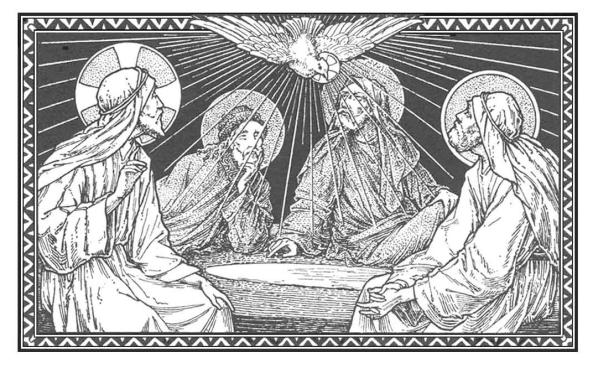
\includegraphics[width=\linewidth]{1.jpg}
\end{figure}

\section{SOBOTA W WIGILIĘ ZESŁANIA DUCHA ŚWIĘTEGO}
 {\station{Stacja u św. Jana na Lateranie}}


\rubric{„Wtedy wrócili do Jerozolimy z góry, zwanej Oliwną, która leży blisko
	Jerozolimy, w odległości drogi szabatowej. Przybywszy tam weszli do sali na
	górze i przebywali w niej: Piotr i Jan, Jakub i Andrzej, Filip i Tomasz,
	Bartłomiej i Mateusz, Jakub, syn Alfeusza, i Szymon Gorliwy, i Juda, brat
	Jakuba. Wszyscy oni trwali jednomyślnie na modlitwie razem z niewiastami,
	Maryją, Matką Jezusa, i braćmi Jego.” (Dz 1, 12-14)

	\medskip

	Wigilia Pięćdziesiątnicy to wyjątkowy obchód w tradycyjnym rycie rzymskim.
	Tego dnia, podobnie jak w czasie Wigilii Paschalnej, dokonuje się
	poświęcenia źródła chrzcielnego i udziela się sakramentów chrztu i
	bierzmowania. Tradycja udzielania tych sakramentów w Wigilie
	Pięćdziesiątnicy pochodzi z pierwszych wieków chrześcijaństwa. Wspominają o
	tym w swoich pismach papieże św. Syrycjusz (384-399) i św. Leon I (440-461),
	powołując się na przykład św. Piotra, który w dzień Zesłania Ducha Świętego
	ochrzcił trzy tysiące osób.}

\newpage

\oremus{Hymn do Ducha Świętego}{
	1. O Stworzycielu Duchu przyjdź,\\
	Nawiedź dusz wiernych Tobie krąg,\\
	Niebieską łaskę zesłać racz,\\
	Sercom, co dziełem są Twych rąk.\\

	2. Pocieszycielem jesteś zwan,\\
	I Najwyższego Boga dar,\\
	Tyś namaszczeniem naszych dusz,\\
	Zdrój żywy, miłość, ognia żar.\\

	3. Ty darzysz łaską siedmiokroć.\\
	Bo moc prawicy Ojca masz,\\
	Przez Ojca obiecany nam,\\
Mową wzbogacasz język nasz.\\}{

	4.Światłem rozjaśnij naszą myśl,\\
	W serca nam miłość świętą wlej,\\
	I wątłą słabość naszych ciał,\\
	Pokrzep stałością mocy Swej.\\

	5. Nieprzyjaciela odpędź w dal,\\
	I Twym pokojem obdarz wraz,\\
	Niech w drodze za przewodem Twym,\\
Miniemy zło co kusi nas.\\

	6. Daj nam przez Ciebie Ojca znać,\\
	Daj, by i Syn poznany był,\\
	I Ciebie jedno Tchnienie Dwóch,\\
	Niech wyznajemy z wszystkich sił.\\}

% \vspace*{-2em}

\begin{center}
	7. Niech Bogu Ojcu chwała brzmi,\\
	Synowi, który zmartwychwstał,\\
	I Temu co pociesza nas,\\
	Niech hołd wieczystych płynie chwał — Amen.
\end{center}

\subsection{LITURGIA SŁOWA --- PROROCTWA}

\rubric{Po odmówieniu Nony w chórze, Kapłan i usługujący w szatach koloru
	fioletowego udają się procesyjnie do ołtarza, oddając mu cześć w zwykły
	sposób, kapłan całuje ołtarz na środku. Następnie odczytuje się proroctwa
	bez tytułu, świece na ołtarzu są zgaszone aż do początku Mszy podobnie jak w
	Wielką Sobotę. Na końcu proroctw odmawia się orację bez \textit{Flectámus
		génua}. 


	Wybrane z kart Starego Testamentu czytania ukazują stopniowy rozwój dzieła
	Odkupienia i zapowiadają odrodzenie w Chrystusie i zesłanie Ducha
	Pocieszyciela. Jest to przygotowanie do poświęcenia wody chrzcielnej, w
	której źródle zaczyna się odrodzenie i nawrócenie człowieka.}

\proroctwoo{Proroctwo I (Rdz 22, 1--19)}{Ofiara Abrahama}

\rubric{Pierwsze proroctwo to fragment Księgi Rodzaju. Ukazuje on heroiczną
	wiarę Abrahama, który wystawiony na bardzo ciężką próbę okazuje całkowite
	posłuszeństwo Bogu. Mądrość Abrahama nie jest mądrością ludzką, opartą o
	wybór tego, co słuszne według rozumu, ale prawdziwą pochodzącą od Boga
	mądrością, która nakazuje zaufać Stwórcy ze względu na jego Boski
	Autorytet.}

% Pierwsze czytanie
W owych dniach Bóg wystawił Abrahama na próbę i rzekł do niego: «Abrahamie!» A
gdy on odpowiedział: «Oto jestem» powiedział: «Weź twego syna jedynego, którego
miłujesz, Izaaka, idź do kraju Moria i tam złóż go w ofierze na jednym z
pagórków, jakie ci wskażę». Nazajutrz rano Abraham osiodłał swego osła, zabrał z
sobą dwóch swych ludzi i syna Izaaka, narąbał drzewa do spalenia ofiary i ruszył
w drogę do miejscowości, o której mu Bóg powiedział. Na trzeci dzień Abraham,
spojrzawszy, dostrzegł z daleka ową miejscowość. I wtedy rzekł do swych sług:
«Zostańcie tu z osłem, ja zaś i chłopiec pójdziemy tam, aby oddać pokłon Bogu, a
potem wrócimy do was». Abraham, zabrawszy drwa do spalenia ofiary, włożył je na
syna swego Izaaka, wziął do ręki ogień i nóż, po czym obaj się oddalili. Izaak
odezwał się do swego ojca Abrahama: «Ojcze mój!» A gdy ten rzekł: «Oto jestem,
mój synu» - zapytał: «Oto ogień i drwa, a gdzież jest jagnię na całopalenie?»
Abraham odpowiedział: «Bóg upatrzy sobie jagnię na całopalenie, synu mój». I
szli obydwaj dalej. A gdy przyszli na to miejsce, które Bóg wskazał, Abraham
zbudował tam ołtarz, ułożył na nim drwa i związawszy syna swego Izaaka położył
go na tych drwach na ołtarzu. Potem Abraham sięgnął ręką po nóż, aby zabić swego
syna. Ale wtedy Anioł Pański zawołał na niego z nieba i rzekł: «Abrahamie,
Abrahamie!» A on rzekł: «Oto jestem». Odpowiedział mu: «Nie podnoś ręki na
chłopca i nie czyń mu nic złego! Teraz poznałem, że boisz się Boga, bo nie
odmówiłeś Mi nawet twego jedynego syna». Abraham, obejrzawszy się poza siebie,
spostrzegł barana uwikłanego rogami w zaroślach. Poszedł więc, wziął barana i
złożył w ofierze całopalnej zamiast swego syna. I dał Abraham miejscu temu nazwę
"Pan widzi". Stąd to mówi się dzisiaj: «Na wzgórzu Pan się ukazuje». Po czym
Anioł Pański przemówił głośno z nieba do Abrahama po raz drugi: «Przysięgam na
siebie, wyrocznia Pana, że ponieważ uczyniłeś to, a nie oszczędziłeś syna twego
jedynego, będę ci błogosławił i dam ci potomstwo tak liczne jak gwiazdy na
niebie i jak ziarnka piasku na wybrzeżu morza; potomkowie twoi zdobędą warownie
swych nieprzyjaciół. Wszystkie ludy ziemi będą sobie życzyć szczęścia [takiego,
jakie jest udziałem] twego potomstwa, dlatego że usłuchałeś mego rozkazu».
Abraham wrócił do swych sług i wyruszywszy razem z nimi w drogę, poszedł do
Beer-Szeby. I mieszkał Abraham nadal w Beer--Szebie.

\oremus{Modlitwa}{Deus, qui in Abrahæ fámuli tui opere humáno generi ob\oe
	diéntiæ exémpla præbuísti; concéde nobis, et nostræ voluntátis pravitátem
	frángere, et tuórum præceptórum rectitúdinem in ómnibus adimplére. Per
	Dóminum nostrum.\\} {Boże, któryś w ofierze sługi swego, Abrahama, dał
	ludziom przykład posłuszeństwa, spraw abyśmy przełamali złość naszej woli i
	we wszystkim wypełniali prawe przykazania Twoje.}

\newpage

\proroctwoo{Proroctwo II (Wj 14, 24--31; 15, 1)}{Przejście Izraela przez Morze
	Czerwone}

\rubric{Drugie proroctwo Wigilii Pięćdziesiątnicy opisuje Przejście Izraelitów
	przez Morze Czerwone. Było ono warunkiem wyzwolenia Izraelitów z niewoli
	egipskiej i wprowadzenia do Ziemi Obiecanej. Jest to zapowiedź chrztu
	świętego, który wyzwala chrześcijan z jarzma szatana i wprowadza do Świętego
	Kościoła.}

W owych dniach o świcie spojrzał Pan ze słupa ognia i ze słupa obłoku na wojsko
egipskie i zmusił je do ucieczki. I zatrzymał koła ich rydwanów, tak że z wielką
trudnością mogli się naprzód posuwać. Egipcjanie krzyknęli: «Uciekajmy przed
Izraelem, bo w jego obronie Pan walczy z Egipcjanami». A Pan rzekł do Mojżesza:
«Wyciągnij rękę nad morze, aby wody zalały Egipcjan, ich rydwany i
jeźdźców».Wyciągnął Mojżesz rękę nad morze, które o brzasku dnia wróciło na
swoje miejsce. Egipcjanie uciekając biegli naprzeciw falom, i pogrążył ich Pan w
środku morza. Powracające fale zatopiły rydwany i jeźdźców całego wojska
faraona, którzy weszli w morze, ścigając tamtych, nie ocalał z nich ani jeden.
Izraelici zaś szli po suchym dnie morskim, mając mur wodny po prawej i po lewej
stronie. W tym to dniu wybawił Pan Izraela z rąk Egipcjan. I widzieli Izraelici
martwych Egipcjan na brzegu morza. Gdy Izraelici widzieli wielkie dzieło,
którego dokonał Pan wobec Egipcjan, ulękli się Pana i uwierzyli Jemu oraz Jego
słudze Mojżeszowi. Wtedy Mojżesz i Izraelici razem z nim śpiewali taką pieśń ku
czci Pana:

\oremus{Pieśń Izraelitów (Wj 15:1--2)}{Cantémus Dómino: glorióse enim
	honorificátus est: equum et ascensórem projécit in mare: adjútor et
	protéctor factus est mihi in salútem, protéctor factus est mihi in
	salútem,\\
	\vv Hic Deus meus, et honorificábo eum: Deus patris mei, et exaltábo eum.\\
	\\
	\vv Dóminus cónterens bella: Dóminus nomen est illi.\\}
{Śpiewajmy Panu, bo bardzo się wsławił, konie i jeźdźców wtrącił w morze. Stał
	się wspomożycielem i obrońcą i wybawił mnie.\\ \\
	\vv On Bogiem moim, więc chwalić Go będę, Bogiem ojca mego, więc będę Go
	sławić.\\
	\vv Pan wiedzie boje. PAN jest imię Jego.}

\oremus{Modlitwa}{Deus, qui primis tempóribus impléta mirácula novi Testaménti
	luce reserásti, ut et Mare Rubrum forma sacri fontis exsísteret, et liberáta
	plebs ab Ægyptíaca servitúte christiáni pópuli  sacraménta præférret: da, ut
	omnes gentes, Israélis privilégium mérito fídei consecútæ, Spíritus tui
	participatióne regeneréntur.} {Boże, który światłem Nowego Testamentu
	wyjaśniłeś cuda czasów poprzednich, abyśmy w Morzu Czerwonym widzieli figurę
	świętej wodzy chrzcielnej, a w ludzie wyzwolonym z niewoli egipskiej figurę
	ludu chrześcijańskiego, przyjmującego święte Sakramenty, daj, niech
	wszystkie  narody przez wiarę zasłużą na dostąpienie przywileju Izraela i
	przez udzielenie im Ducha Świętego zostaną w jedności Tegoż odrodzone.}

\proroctwoo{Proroctwo III (Pwt 31,22--30)}{Napomnienie Mojżesza}

\rubric{Trzecie proroctwo Wigilii Pięćdziesiątnicy to pouczenie, jakie Mojżesz
	skierował do Izraelitów. Kościół kieruje je do wszystkich przygotowujących
	się do Chrztu świętego oraz do wszystkich ochrzczonych. Wzywa ono lud, aby
	zachował wierność swojemu Bogu.}

Mojżesz napisał tę pieśń w owym dniu i nauczył jej Izraelitów. Pan dał taki
rozkaz Jozuemu, synowi Nuna: «Bądź mężny i mocny, gdyż ty zaprowadzisz
Izraelitów do ziemi, którą im poprzysiągłem, a Ja będę z tobą». Gdy Mojżesz
zakończył całkowicie pisanie tego Prawa w księdze, rozkazał lewitom noszącym
Arkę Przymierza Pańskiego: «Weźcie tę Księgę Prawa i połóżcie ją obok Arki
Przymierza Pana, Boga waszego, a niech tam będzie przeciwko wam jako świadek. Ja
bowiem znam wasz upór i twardy kark. Oto jak długo żyję z wami, opornie
postępowaliście względem Pana. Cóż dopiero po mojej śmierci?» «Zbierzcie u mnie
wszystkich starszych z waszych pokoleń i zwierzchników, abym powiedział do ich
uszu te słowa i wezwał przeciw nim niebo i ziemię na świadków. Ponieważ wiem, że
po mojej śmierci na pewno w przyszłości sprzeniewierzycie się i odstąpicie od
drogi, którą wam przykazałem. Dosięgnie was nieszczęście, gdy czynić będziecie
to, co jest złe w oczach Pana, gniewając Go czynami rąk waszych». Potem wygłosił
Mojżesz do uszu całej społeczności Izraela wszystkie słowa tej pieśni:

\oremus{Pieśń Mojżesza (Pp 32:1--4)}{Atténde, cœlum, et loquar: et áudiat terra
	verba ex ore meo.\\
	\vv Exspectétur sicut plúvia elóquium meum: et descéndant sicut ros verba
	mea.\\
	\vv Sicut imber super gramen et sicut nix super fænum: quia nomen Dómini
	invocábo,\\
	\vv Date magnitúdinem Deo nostro: Deus, vera ópera ejus, et omnes viæ ejus
	judícia,\\ \\
	\vv Deus fidélis, in quo non est iníquitas: justus et sanctus
	Dóminus.}{Słuchajcie, niebiosa, a będę mówił, niech słucha ziemia mowy ust
	moich.\\
	\vv Niech spływa jak deszcz nauka moja i niech zstąpią jak rosa słowa
	moje.\\
	\vv Jak ulewa na trawę i jak krople dżdżu na zioła, gdyż imię Pańskie
	opiewać będę.\\\\
	\vv Oddajcie chwałę Bogu naszemu. Dzieła Boże są doskonałe, a wszystkie
	drogi Jego sprawiedliwe.\\
	\vv Bóg wierny i bez skazy, Pan sprawiedliwy i święty.}

\newpage

\oremus{Modlitwa}{Deus, qui glorificátio fidélium et vita justórum, qui per
	Móysen, fámulum tuum, nos quoque modulatióne sacri cárminis erudísti:
	univérsis géntibus misericórdiæ tuæ munus operáre, tribuéndo beatitúdinem,
	auferéndo terrórem; ut, quod pronuntiátum est ad supplícium, in remédium
	transferátur ætérnum. Per Dóminum.}{Boże, chwało wiernych i żywocie
	sprawiedliwych, któryś przez sługę swojego, Mojżesza, pouczył nas śpiewem
	hymnu świętego, dokonaj nad wszystkimi narodami dzieła miłosierdzia swego,
	darząc szczęśliwością, oddalając trwogę, aby to, co było zapowiedzią kary,
	stało się lekarstwem na wieczność.}

\proroctwoo{Proroctwo IV (Iz 4,1--6)}{Odrośl Pana}

\rubric{Czwarte proroctwo Wigilii Pięćdziesiątnicy to fragment Księgi Proroka
	Izajasza. Ocalona z pogromu cząstka Izraela stała się wybraną winnicą Bożą.
	Przez cierpienia Bóg oczyścił winy narodu i otoczył go troskliwą opieką.
	Podobnie spośród ludzkości Pan Bóg wybiera członków swojego Kościoła, który
	jest dzisiaj wybraną winnicą Bożą.}

Siedem niewiast uchwyci się jednego mężczyzny w ów dzień, mówiąc: «Swój chleb
będziemy jadły i we własną odzież się ubierały. Dozwól nam tylko nosić twoje
imię. Odejmij nam hańbę». W owym dniu Odrośl Pana stanie się ozdobą i chwałą, a
owoc ziemi przepychem i krasą dla ocalałych z Izraela. I będzie tak: Ten, kto
pozostał żywy na Syjonie, i który się ostał w Jeruzalem, każdy będzie nazwany
świętym i wpisany do Księgi Życia w Jeruzalem. Gdy Pan obmyje brud Córy
Syjońskiej i krew rozlaną oczyści wewnątrz Jeruzalem tchnieniem sądu i
tchnieniem pożogi, wtedy Pan przyjdzie spocząć na całej przestrzeni góry Syjonu
i na tych, którzy się tam zgromadzą, we dnie jak obłok z dymu, w nocy jako
olśniewający płomień ognia. Albowiem nad wszystkim Chwała Pańska będzie osłoną i
namiotem, by za dnia dać cień przed skwarem, ucieczkę zaś i schronienie przed
nawałnicą i ulewą.

\oremus{Pieśń Izajasza (Iz 5:1--2)}{Vínea facta est dilécto in cornu, in loco
	úberi.\\
	\vv Et macériam circúmdedit, et circumfódit: et plantávit víneam Sorec, et
	ædificávit turrim in médio ejus.\\
	\vv Et tórcular fodit in ea: vínea enim Dómini Sábaoth domus Israël
	est.}{Winnicę miał mój przyjaciel na urodzajnym wzgórzu.\\
	\vv I skopał ją, i oczyścił z kamieni, i zasadził w niej winorośl wyborną, i
	pośrodku wieżę zbudował.\\
	\vv I wykuł tam także tłocznię. Winnicą Pana Zastępów jest dom Izraela.}

\oremus{Modlitwa}{Omnípotens sempitérne Deus, qui, per únicum Fílium tuum,
	Ecclésiæ tuæ demonstrásti te esse cultórem, omnem pálmitem, fructum in eodem
	Christo tuo, qui vera vitis est, afferéntem, cleménter éxcolens, ut fructus
	áfferat amplióres: fidélibus tuis, quos velut víneam ex Ægýpto per fontem
	baptísmi transtulísti, nullæ peccatórum spinæ præváleant; ut, Spíritus tui
	sanctificatióne muníti, perpétua fruge diténtur. Per eúndem Dóminum . . . in
	unitáte ejusdem.}{Wszechmogący, wieczny Boże, który przez Jednorodzonego
	Syna swego okazałeś się tym, który uprawia rolę Kościoła, gdyż wszelką
	gałązkę przynoszącą owoc W Chrystusie, który jest prawdziwą winną latoroślą,
	z miłością pielęgnujesz, aby wydała owoc obfitszy; spraw niech ciernie
	grzechowe nie wzrastają wpośród Tych wiernych, których jako winnicę z Egiptu
	przez wodę Chrztu przeniosłeś, aby, umocnieni Duchem Poświęcicielem,
	obfitowali w dobra wieczne.}

\proroctwoo{Proroctwo V (Ba 3,9--38)}{Mądrością jest księga przykazań Boga}

\rubric{Liturgia przytacza nam mowę Proroka Barucha do przerażonych Izraelitów.
	Prorok poucza ich, co powinni czynić , by ż yć w Bożym pokoju. Kościół uczy
	nas, ż e również nasze dusze - dusze ochrzczonych będą się cieszyć
	posiadaniem nieustannego pokoju, o ile zastosują się do życiodajnych i
	pełnych mądrości nauk, których nam Bóg przez swój Święty Kościół udziela.}

\noindent Bądź posłuszny, Izraelu, przykazaniom życiodajnym, \\
nakłoń ucha, by poznać mądrość. \\
Cóż się to stało, Izraelu, \\
że jesteś w kraju nieprzyjaciół, \\
wynędzniały w ziemi obcej, \\
uważany za nieczystego na równi z umarłymi, \\
zaliczony do tych, co schodzą do Szeolu? \\
Opuściłeś źródło mądrości. \\
Gdybyś chodził po drodze Bożej, \\
mieszkałbyś w pokoju na wieki. \\
Naucz się, gdzie jest mądrość, \\
gdzie jest siła i rozum, \\
a poznasz równocześnie, \\
gdzie jest długie i szczęśliwe życie, \\
gdzie jest światłość dla oczu i pokój. \\
Lecz któż znalazł jej miejsce \\
lub kto wszedł do jej skarbców? \\
Gdzież są zwierzchnicy narodów \\
i panujący nad zwierzętami ziemi, \\
ci, co igrają z ptakami powietrznymi, \\
ci, co gromadzą srebro i złoto, \\
w których ludzie złożyli ufność, \\
a nie ma końca nabywaniu tych rzeczy, \\
którzy obrabiają srebro, \\
trudzą się, tak że prawie nie kończy się ich praca? \\
Zniknęli i do Szeolu zstąpili, \\
a inni stanęli na ich miejsce. \\
Młodsi ujrzeli światło \\
i zamieszkali na ziemi, \\
ale drogi mądrości nie pojęli, \\
nie poznali jej ścieżek \\
ani jej nie uchwycili, \\
a synowie ich od drogi swej daleko odeszli. \\
Nie słyszano o niej w Kanaanie\\
ani w Temanie jej nie widziano. \\
Synowie Hagar ubiegają się o mądrość tej ziemi,\\
kupcy Merranu i Temanu, opowiadający baśnie i poszukiwacze wiedzy, \\
drogi mądrości nie znają \\
ani nie pamiętają o jej ścieżkach. \\
O Izraelu, jakże wielki jest dom Boga, \\
jakże obszerne miejsce posiadłości Jego!  Wielki i nie mający końca, \\
wysoki i niezmierzony. \\
Tam urodzili się olbrzymi, \\
sławni od początku, \\
wielcy, biegli w walce. \\
Ale nie tych wybrał Bóg \\
ani im nie dał drogi do mądrości. \\
Zginęli dlatego, że mądrości nie mieli, \\
zginęli z powodu swej nierozwagi. \\
Któż wstąpił do nieba, aby ją wziąć, \\
któż ją z obłoków sprowadził? \\
Któż przeprawił się przez morze, a znalazł ją \\
i przywiózł ją w zamian za najlepsze złoto? \\
Nie ma nikogo, kto by znał jej drogę \\
i kto by rozpoznał jej ścieżkę. \\
Lecz zna ją Wszechwiedzący \\
i wynajdzie ją swoją mądrością. \\
Ten, który na czas bezkresny urządził ziemię \\
i napełnił ją stworzeniami czworonożnymi, \\
wysłał światło i poszło, \\
wezwał je, a ono posłuchało Go ze drżeniem. \\
Gwiazdy radośnie świecą na swoich strażnicach.\\
Wezwał je. Odpowiedziały: «Jesteśmy». \\
Z radością świecą swemu Stwórcy. \\
On jest Bogiem naszym. \\
I żaden inny nie może \\
z Nim się równać. \\
Zbadał wszystkie drogi mądrości \\
i dał ją słudze swemu, Jakubowi, \\
i Izraelowi, umiłowanemu swojemu. \\
Potem ukazała się ona na ziemi \\
i zaczęła przebywać wśród ludzi.

\oremus{Modlitwa}{Deus, qui nobis per Prophetárum ora præcepísti temporália
	relínquere atque ad ætérna festináre: da fámulis tuis; ut, quæ a te jussa
	cognóvimus, implére c\oe lésti inspiratióne valeámus. Per Dóminum.}{Boże,
	któryś nam przez usta proroków nakazał opuszczać dobra ziemskie, a kwapić
	się ku wiecznym, daj sługom Twoim, abyśmy, znając Twe przykazania,
	wypełniali je z pomocą łaski Twej świętej.}

\proroctwoo{Proroctwo VI (Ez 37,1--14)}{Wizja wyschniętych kości}

\rubric{Prorok opisuje wizję ożywienia wysuszonych kości. Jak w widzeniu
	Ezechiela, na rozkaz proroka kości zeschłe przyoblekają się w ciało i stają
	się wojskiempotężnym, tak dusze nasze przez Chrzest święty otrzymują nowe
	życie.}

W owych dniach spoczęła na mnie ręka Pana, i wyprowadził mnie On w duchu na
zewnątrz, i postawił mnie pośród doliny. Była ona pełna kości. I polecił mi,
abym przeszedł dokoła nich, i oto było ich na obszarze doliny bardzo wiele. Były
one zupełnie wyschłe. I rzekł do mnie: «Synu człowieczy, czy kości te powrócą
znowu do życia?» Odpowiedziałem: «Panie Boże, Ty to wiesz». Wtedy rzekł On do
mnie: «Prorokuj nad tymi kośćmi i mów do nich: „Wyschłe kości, słuchajcie słowa
Pana!” Tak mówi Pan Bóg: Oto Ja wam daję ducha po to, abyście się stały żywe.
Chcę was otoczyć ścięgnami i sprawić, byście obrosły ciałem, i przybrać was w
skórę, i dać wam ducha po to, abyście ożyły i poznały, że Ja jestem Pan». I
prorokowałem, jak mi było polecone, a gdym prorokował, oto powstał szum i
trzask, i kości jedna po drugiej zbliżały się do siebie. I patrzyłem, a oto
powróciły ścięgna i wyrosło ciało, a skóra pokryła je z wierzchu, ale jeszcze
nie było w nich ducha. I powiedział On do mnie: «Prorokuj do ducha, prorokuj, o
synu człowieczy, i mów do ducha: Tak powiada Pan Bóg: Z czterech wiatrów
przybądź, duchu, i powiej po tych pobitych, aby ożyli». Wtedy prorokowałem tak,
jak mi nakazał, i duch wstąpił w nich, a ożyli i stanęli na nogach – wojsko
bardzo, bardzo wielkie. I rzekł do mnie: «Synu człowieczy, kości te to cały dom
Izraela. Oto mówią oni: „Wyschły kości nasze, minęła nadzieja nasza, już po nas”
. Dlatego prorokuj i mów do nich: Tak mówi Pan Bóg: Oto otwieram wasze groby i
wydobywam was z grobów, ludu mój, i wiodę was do kraju Izraela, i poznacie, że
Ja jestem Pan, gdy wasze groby otworzę i z grobów was wydobędę, ludu mój.
Udzielę wam mego ducha po to, byście ożyli, i powiodę was do kraju waszego, i
poznacie, że Ja, Pan, to powiedziałem i wykonam» – mówi Pan wszechmogący.

\oremus{Modlitwa}{Dómine, Deus virtútum, qui collápsa réparas et reparáta
	consérvas: auge pópulos in tui nóminis sanctificatióne renovándos; ut omnes,
	qui sacro	baptísmate diluúntur, tua semper inspiratióne dirigántur. Per
	Dóminum nostrum.}{Panie, Boże Zastępów, który to, co było upadłe naprawiasz,
	a naprawione zachowujesz, pomnóż ludy odrodzone wyznawaniem Twojego Imienia,
	aby wszyscy, których obmyła woda Chrztu świętego, kierowali się zawsze Twym
	natchnieniem.}

\vspace*{1cm}

\centerline{\pgfornament[width=4cm]{82}}

\vspace*{1cm}

\subsection{LITURGIA CHRZCIELNA}

\rubric{Po zakończeniu proroctw kapłan ubrany w kapę koloru fioletowego udaje
	się procesyjnie do chrzcielnicy,. Procesję prowadzi posługujący z paschałem,
	za nim ministrant z krzyżem, po dwóch jego stronach idą akolici z zapalonymi
	świecami, następnie usługujący, duchowieństwo wg porządku starszeństwa,
	celebrans z diakonem i subdiakonem. W trakcie procesji śpiewa się:}

\oremus{Psalm 41, 2--4}{Sicut cervus desíderat ad fontes aquárum: iía desíderat
	ánima mea ad te, Deus. \\
	\vv Sitívit ánima mea ad Deum vivum: quando véniam, et apparébo ante fáciem
	Dei? \\
	\vv Fuérunt mihi lácrimæ meæ panes die ac nocte, dum dícitur mihi per
	síngulos dies: Ubi est Deus tuus?\\}{Jak jeleń spragniony dąży do strumieni
	wody, tak dusza ma tęskni za Tobą, Boże.\\ \vv Tęskni ma dusza za Bogiem
	żywym, kiedyż przyjdę i stanę przed Bożym obliczem?\\
	\vv Łzy moje są mi pokarmem we dnie i w nocy, gdy mówią do mnie co dzień
	«Gdzież jest twój Bóg?»}

%				\newpage

\oremus{Modlitwa na progu baptysterium}{
	\vv Dóminus vobíscum. \\
	\rr Et cum spíritu tuo.\\
	Orémus.\\
	Concéde, quǽsumus, omnípotens Deus: ut, qui sollemnitátem doni Sancti
	Spíritus cólimus, c\oe léstibus desidériis accénsi, fontem vitæ sitiámus.Per
	ómnia sǽcula sæculórum.\\
	\rr Amen.}{
	\vv Pan z Wami.\\
	\rr I z duchem Twoim.\\
	Módlmy się\\
	Daj, prosimy Cię, wszechmogący Boże, abyśmy święcąc uroczystość Zesłania
	Ducha Świętego, niebieską żądzą zapaleni, pragnęli zdroju żywota.Przez
	wszystkie wieki wieków.\\
	\rr Amen.}

\oremus{Poświęcenie wody chrzcielnej}{
	\vv Dóminus vobíscum.\\
	\rr Et cum spiritu tuo.\\
	Orémus.\\
	Omnípotens sempitérne Deus, adésto magnæ pietátis tuæ mystériis, adésto
	sacraméntis: et ad recreándos novos pópulos, quos tibi fons baptismátis
	párturit, spíritum adoptiónis emítte ; ut, quod nostræ humilitátis geréndum
	est ministério, virtútis tuæ impleátur efféctu. Per Dóminum nostrum Iesum
	Christum, Fílium tuum: Qui tecum vivit et regnat in unitáte Spíritus Sancti
	Deus: per Omnia s\ae cula S\ae culorum. \\ \\
	\vv Amen.\\
	\vv Dóminus vobíscum.\\
	\rr Et cum spíritu tuo.\\
	\vv Sursum corda.\\
	\rr Habémus ad Dóminum.\\
	\vv Grátias agámus Dómino Deo nostro.\\
	\rr Dignum et iustum est.\\
	Vere dignum et iustum est, æquum et salutare, nos tibi semper et ubique
	gratias agere, Domine, sancte Pater, omnipotens æterne Deus: qui invisibili
	potentia, sacramentorum tuorum mirabiliter operaris effectum: et licet nos
	tantis mysteriis exsequendis simus indigni: tu tamen gratiæ tuæ dona non
	deserens, etiam ad nostras preces aures tuæ pietatis inclinas. Deus, cuius
	Spiritus super aquas inter ipsa munda primordia ferebatur: ut iam tunc
	virtutem sanctificationis, aquarum natura conciperet. Deus, qui nocentis
	mundi crimina per aquas abluens, regenerationis speciem in ipsa diluvii
	effusione signasti: ut, unius eiusdemque elementi mysterio, et finis esset
	vitiis, et origo virtutibus. Respice, Domine, in faciem Ecclesiæ tuæ, et
	multiplica in ea regenerationes tuas, qui gratiæ tuæ affluentis impetu
	lætificas civitatem tuam: fontemque baptismatis aperis toto orbe terrarum
	gentibus innovandis: ut, tuæ maiestatis imperio, sumat Unigeniti tui gratiam
	de Spiritu Sancto.}{\vv Pan z wami.\\
	\rr I z duchem twoim.\\
	Módlmy się.\\
	Wszechmogący, wiekuisty Boże, bądź obecny w tych tajemnicach Twej wielkiej
	dobroci, bądź obecny w sakramentach i ześlij ducha przybrania, aby dać nowe
	życie ludowi, który rodzi się w źródle chrzcielnym. Spraw, aby poświęcenie,
	które ma się dokonać przez naszą niegodną posługę, otrzymało skuteczność
	dzięki Twojej mocy. Przez Pana naszego Jezusa Chrystusa, Syna Twojego, który
	z Tobą żyje i króluje w jedności Ducha Świętego, Bóg przez wszystkie wieki
	wieków.\\
	\vv Amen. \\
	\vv Pan z wami.\\
	\rr I z duchem twoim.\\
	\vv W górę serca.\\
	\rr Wznieśliśmy je ku Panu.\\
	\vv Dzięki składajmy Panu, Bogu naszemu.\\
	\rr Godne to i sprawiedliwe.\\
	Zaprawdę godne to i sprawiedliwe, słuszne i zbawienne, abyśmy zawsze i
	wszędzie Tobie składali dziękczynienie, Panie, Ojcze święty, wszechmogący
	wieczny Boże! Twoja niewidzialna moc  nadaje sakramentom cudowną skuteczność
	i chociaż jesteśmy niegodni sprawować tak wielkie tajemnice, Ty nie
	zapominasz o darach Twej łaski i skłaniasz miłościwie ucho nawet ku naszym
	prośbom. Duch Twój, o Boże, unosił się nad wodami w samym zaraniu świata,
	aby już wtedy żywioł wody otrzymał zaczątek mocy uświęcania. Boże, Ty
	obmywając wodą zbrodnie występnego świata, potop uczyniłeś obrazem mającego
	nadejść odrodzenia przez Chrzest, ten sam bowiem żywioł wody w tajemniczy
	sposób kładzie kres występkom i stanowi początek cnót. Wejrzyj, Panie, na
	oblicze Kościoła Twojego i pomnóż w nim zastęp Twych dzieci. Ty rozweselasz
	królestwo Twoje obfitym strumieniem Swoich łask i otwierasz źródło
	chrzcielna do odrodzenia ludów pogańskich na całej kuli ziemskiej. Niech z
	woli Twego majestatu woda ta otrzyma łaskę Twego Jednorodzonego Syna z Ducha
	Świętego.}

\rubric{
	Czyni dłonią znak krzyża na wodzie, wyciera dłonie w ręcznik i kontynuuje:}

\oremuss{Qui hanc aquam, regenerandis hominibus præparatam, arcana sui numinis
	admixtione fecundet: ut, sanctificatione concepta, ab immaculato divini
	fontis utero, in novam renata creaturam, progenies cælestis emergat: et quos
	aut sexus in corpore, aut ætas discernit in tempore, omnes in unam pariat
	gratia mater infantiam. Procul ergo hinc, iubente te, Domine, omnis spiritus
	immundus abscedat: procul tota nequitia diabolicæ fraudis absistat. Nihil
	hoc loci habeat contrariæ virtutis admixtio: non insidiando cicumvolet: non
	latendo subrepat: non inficiendo corrumpat.}{Niech Duch Święty przez
	tajemnicze działanie swej mocy uczyni płodną tę wodę przygotowaną do
	odrodzenia ludzi, aby z czystego łona tego Bożego źródła wynurzyło się
	niebiańskie pokolenie poczęte w świętości i zrodzone do nowego życia. Niech
	łaska jak matka zrodzi ich do jednego dziecięctwa, mimo różnic płci i wieku.
	Niech więc, o Panie, na Twój rozkaz precz stąd uchodzi wszelki duch
	nieczysty, niech precz odstąpi cała przewrotność zdradzieckiego szatana.
	Niech nie znajdzie tu przystępu wpływ wrażej mocy, niech nie krąży ona
	gotując zasadzki, niech się nie wkrada po kryjomu, niech się nie waży psuć i
	zarażać.}

\rubric{Dotyka ręką wody.}

\oremuss{Sit hæc sancta et innocens creatura, libera ab omni impugnatoris
	incursu, et totius nequitiæ purgata discessu. Sit fons vivus, aqua
	regenerans, unda purificans: ut omnes hoc lavacro salutifero diluendi,
	operante in eis Spiritu Sancto, perfectæ purgationis indulgentiam
	consequantur. }{Niech to święte i niewinne stworzenie będzie wolne od
	wszelkiej napaści przeciwnika i oczyszczone przez usunięcie wszelkiej
	nieprawości. Niech będzie źródłem życia, wodą odradzającą, falą
	oczyszczającą, aby wszyscy, którzy zostaną obmyci w tej zbawiennej kąpieli,
	otrzymali łaskę doskonałego oczyszczenia za sprawą Ducha Świętego.}

\rubric{Czyni trzy znaki krzyża nad wodą mówiąc:}

\oremuss{Unde benedico te, creatura aquæ, per Deum \cross vivum, per Deum
	\cross verum, per Deum \cross sanctum: per Deum, qui te, in principio,
	verbo separavit ab arida: cuius Spiritus super te ferebatur. }{Przeto
	błogosławię cię, wodo, w imię Boga \cross żywego, w imię Boga \cross
	prawdziwego, w imię Boga \cross świętego, w imię Boga, który na początku
	słowem oddzielił cię od suchej ziem, którego Duch unosił się nad tobą.}

\rubric{Ręką rozdziela wodę i rozlewa ją na cztery strony świata.}

\oremuss{Qui te paradisi fonte manare fecit, et in quatuor fluminibus totam
	terram rigare præcepit. Qui te in deserto amaram, suavitate indita, fecit
	esse potabilem, et sitienti populo de petra produxit. Bene ☩ dico te et per
	Iesum Christum Filium eius unicum, Dominum nostrum: qui te in Cana Galilææ
	signo admirabili, sua potentia convertit in vinum. Qui pedibus super te
	ambulavit: et a Ioanne in Iordane in te baptizatus est. Qui te una cum
	sanguine de latere suo produxit: et discipulis suis iussit, ut credentes
	baptizarentur in te, dicens: Ite, docete omnes gentes, baptizantes eos in
	nomine Patris, et Filii, et Spiritus Sancti. }{
	\vspace*{-2pt}
	On to sprawił, żeś wytrysnęła z rajskiego źródła i czterema strumieniami
	zrosiła całą ziemię; On to na puszczy, gdyś była gorzką, przemienił cię w
	słodką i zdatną do picia oraz wyprowadził cię ze skały dla napojenia
	spragnionego ludu. Błogo ☩ sławię cię w imię Jezusa Chrystusa, Jego Jedynego
	Syna a Pana naszego, który w Kanie Galilejskiej przemienił cię w wino
	przedziwnym cudem swej potęgi. On to własnymi stopami chodził po tobie i w
	twoich falach został ochrzczony przez Jana w Jordanie. On cię wytoczył ze
	Swego boku razem z krwią, uczniom swoim kazał tobą chrzcić wierzących,
	mówiąc : «Idźcie i nauczajcie wszystkie narody, chrzcząc je w imię Ojca i
	Syna, i Ducha Świętego. }

%				\newpage

\rubric{Następnie czytając (lub w tonie lekcji) kontynuuje:}

\oremuss{Hæc nobis præcépta servantibus, tu, Deus omnípotens, clemens adésto: tu
	benignus aspíra.}{Gdy będziemy spełniać to przykazanie, Ty, Boże
	wszechmogący, przybądź nam łaskawie z pomocą i w dobroci Twojej ześlij
	tchnienie Twego Ducha. }

\rubric{Tchnie trzykrotnie w kształcie krzyża \cross i mówi:}

\oremuss{Tu has simplices aquas tuo ore benedicito: ut præter naturálem
	emundatiónem, quam lavándis possunt adhibere corpóribus, sint etiam
	purificándis méntibus efficáces.}{Pobłogosław tę czystą wodę tchnieniem
	Twoich ust, aby oprócz naturalnej właściwości oczyszczania ciał tych, którzy
	się nią myją, otrzymała moc oczyszczania dusz. }

\rubric{Wstawiając paschał do wody śpiewa w tonie prefacji:}

\oremuss{
	Descendat in hanc plenitudinem fontis virtus Spiritus Sancti.}{
	Niech moc Ducha Świętego zstąpi w wodę wypełniającą to źródło chrzcielne.}

\rubric{Wyciąga paschał z wody i wstawia go ponownie głębiej powtarzając
	\textit{Descéndat}. Ponownie wyciąga paschał i wstawia po raz trzeci tym
	razem na dno i powtarza \textit{Descéndat}. Następnie trzymając paschał w
	wodzie kapłan tchnie trzykrotnie w wodę formując grecką literę $\Psi$, od
	której rozpoczyna się wyraz PSYCHE, to znaczy dusza: }

\oremuss{
	Totamque huius aquæ substantiam, regenerandi fecundet effectu. }{
	Niech zapłodni całą tę wodę dając jej moc odradzania.}

\rubric{
	Paschał wyjmuje się z wody i odstawia na swoje miejsce. Celebrans kontynuuje:}

\oremuss{Hic omnium peccatorum maculæ deleantur: hic natura ad imaginem tuam
	condita, et ad honorem sui reformata principii, conctis vetustatis
	squaloribus emundetur: ut omnis homo, sacramentum hoc regenerationis
	ingressus, in veræ innocentiæ novam infantium renascatur.}{Niech tutaj
	zostaną obmyte zmazy grzechów. Niech tutaj natura stworzona na Twój obraz i
	przywrócona do pierwotnej godności zostanie oczyszczona od wszelkich
	zastarzałych brudów, aby każdy człowiek, który przystąpi do tego sakramentu
	odrodzenia, odżył jako nowe dziecko w prawdziwej niewinności.}

\rubric{Czytając}

\oremuss{Per Dóminum nostrum Jesum Christum, Fílium tuum: Qui ventúrus est
	judicáre vivos et mórtuos, et sǽculum per ignem\\
	\rr Amen.}{Przez Pana naszego Jezusa Chrystusa, Syna Twego, który przyjdzie
	sądzić żywych i umarłych i świat przez ogień.\\
	\rr Amen}

%				\newpage

\rubric{Jeden z usługujących nabiera wody do osobnego naczynia do kropielnic,
	poświęceń itp. Kapłan kropi wiernych wodą święconą, w tym czasie można
	śpiewać stosowną pieśń.}

\oremus{Pieśń na pokropienie}{
	1. Com przyrzekł Bogu przy chrzcie raz,\\
	Dotrzymać pragnę szczerze.\\
	Kościoła słuchać w każdy czas,\\
	I w świętej wytrwać wierze.\\

	~~~~~Ref.: O Panie Boże, dzięki Ci,

	~~~~~Żeś mi Kościoła otwarł drzwi.

	~~~~~W nim żyć, umierać pragnę.\\}{
	2. W Kościele tym jest z Ciałem, Krwią, \\
	Bóg pod postacią chleba\\
	Swym Ciałem Karmi duszę mą,\\
	By żyła w nim dla nieba.\\

	~~~~~Ref.: W to wierzyć zawsze mocno chcę,

	~~~~~Bo tego kościół uczy mnie.

	~~~~~W nim żyć, umierać, pragnę.\\}

\newpage

\rubric{Do pozostałej części pozostawionej w chrzcielnicy kapłan wlewa Olej
	Katechumenów na kształt krzyża i mówi:}

\oremuss{Sanctificétur et fecundétur fons iste Oleo salútis renascéntibus ex eo,
	in vitam ætérnam.}{Niech Olej zbawienia uświęci tę wodę \cross i da jej moc
	odradzania na życie wieczne. }

\rubric{Wlewa Krzyżmo w podobny sposób jak powyżej i mówi:}

\oremuss{Infúsio Chrísmatis Dómini nostri Jesu Christi, et Spíritus Sancti
	Parácliti, fiat in nómine sanctæ Trinitátis.}{Wlanie Krzyżma Pana naszego
	Jezusa Chrystusa i Ducha Świętego Pocieszyciela niech się dokona w imię
	Trójcy Świętej.}

\rubric{Następnie wlewa jednocześnie Olej Katechumenów oraz Krzyżmo w podobny
	sposób jak powyżej i mówi:}

\oremuss{Commíxtio Chrísmatis sanctificatiónis, et Olei unctiónis, et Aquæ
	baptísmatis, páriter fiat in nómine Pa \cross tris, et Fí \cross lii,
	et Spíritus \cross Sancti.\\
	\rr Amen.}{Zmieszanie Krzyżma uświęcającego, Oleju namaszczenia i wody
	chrzcielnej niechaj się dokona w imię Oj \cross ca i Sy \cross na i
	Ducha \cross Świętego.\\
	\rr Amen }

\vspace*{0.5cm}

\centerline{\pgfornament[width=4cm]{82}}

% \newpage

\subsection{LITANIA DO WSZYSTKICH ŚWIĘTYCH}

\rubric{Po skończonej Liturgii Chrzcielnej rozpoczyna się śpiew litanii do
	wszystkich świętych. Wezwania śpiewa dwóch lub więcej kantorów. Po wezwaniu
	\textit{Sancta Trinitas Unus Deus} kapłan i usługujący procesjonalnie udają
	się do ołtarza. Po powrocie klękają, a kantorzy śpiewają litanię pośrodku
	chóru. W drugiej części Litanii kapłan z usługującymi wstają i udają się do
	zakrystii. W tym czasie zapala się świece i przygotowuje ołtarz do Mszy św.}

% \rubric{Ochrzczeni i bierzmowani podążają za światłem paschału -- Chrystusa
% 	Zmartwychwstałego -- do nawy kościoła i zajmują miejsce pośród wspólnoty
% 	wiernych. Już za chwilę będą mogli z całym Kościołem zaśpiewać wspólne
% 	"Alleluja" i przyjąć Komunię Świętą.}

% \vspace*{2cm}
% \newpage

% \gregorioscore{Melody/kyrie.gabc}
% \vspace*{1em}

\oremuss{\vv Kýrie eléison. \rrr Kýrie eléison. \\
	\vv Christe eléison. \rrr Christe eléison. \\
	\vv Kýrie eléison. \rrr Kýrie eléison.\\}{
	\vv Kyrie, eleison. \rrr Kyrie, eleison.\\
	\vv Christe, eleison. \rrr Christe, eleison. \\
	\vv Kyrie, eleison. \rrr Kyrie, eleison.\\}

% \gregorioscore{Melody/misserere.gabc}
% \vspace*{1em}

\oremuss{\vv Pater de cǽlis, Deus. \rrr Miserére nobis.\\
	\vv Fili Redémptor mundi, Deus. \rrr Miserére nobis.\\
	\vv Spíritus Sancte, Deus. \rrr Miserére nobis.\\
	\vv Sancta Trínitas, unus Deus. \rrr Miserére nobis. \\}{
	\vv Ojcze z nieba, Boże. \rrr Zmiłuj się nad nami.\\
	\vv Synu, Odkupicielu świata, Boże. \rrr Zmiłuj się nad nami.\\
	\vv Duchu Święty, Boże. \rrr Zmiłuj się nad nami.\\
	\vv Święta Trójco, jedyny Boże. \rrr Zmiłuj się nad nami.\\
}

% \gregorioscore{Melody/ora.gabc}
% \vspace*{1em}

\oremuss{
	\vv Sancta María. \rrr Ora pro nobis.\\
	\vv Sancta Dei Génetrix. \rrr Ora pro nobis.\\
	\vv Sancta Virgo vírginum. \rrr Ora pro nobis.\\
	\vv Sancte Míchaël. \rrr Ora pro nobis.\\
	\vv Sancte Gábriel. \rrr Ora pro nobis.\\
	\vv Sancte Ráphaël. \rrr Ora pro nobis.\\
	\vv Omnes sancti Angeli et Archángeli.\\ \rrr Oráte pro nobis.\\
	\vv Omnes sancti beatórum Spirítuum órdines. \rrr Oráte pro nobis.\\
	\vv Sancte Ioánnes Baptísta. \rrr Ora pro nobis.\\
	\vv Sancte Ioseph. \rrr Ora pro nobis.\\
	\vv Omnes sancte Patriárchæ et Prophétæ.\\ \rrr Oráte pro nobis. \\
	\vv Sancte Petre. \rrr Ora pro nobis.\\
	\vv Sancte Paule. \rrr Ora pro nobis.\\
	\vv Sancte Andréa. \rrr Ora pro nobis.\\
	\vv Sancte Ioánnes. \rrr Ora pro nobis.\\
	\vv Omnes sancti Apóstoli et Evangelístæ. \\\rrr Oráte pro nobis.\\
	\vv Omnes sancti Discípuli Dómini. \rrr Oráte pro nobis.\\
	\vv Sancte Stéphane. \rrr Ora pro nobis.\\
	\vv Sancte Laurénti. \rrr Ora pro nobis.\\
	\vv Sancte Vincénti. \rrr Ora pro nobis.\\
	\vv Omnes sancti Mártyres. \rrr Oráte pro nobis. \\
	\vv Sancte Silvéster. \rrr Ora pro nobis.\\
	\vv Sancte Gregóri. \rrr Ora pro nobis.\\
	\vv Sancte Augustíne. \rrr Ora pro nobis.\\
	\vv Omnes sancti Pontífices et Confessóres. \rrr Oráte pro nobis.\\
	\vv Omnes sancti Doctóres. \rrr Oráte pro nobis.\\
	\vv Sancte Antóni. \rrr Ora pro nobis.\\
	\vv Sancte Benedícte. \rrr Ora pro nobis.\\
	\vv Sancte Domínice. \rrr Ora pro nobis.\\
	\vv Sancte Francísce. \rrr Ora pro nobis.\\
	\vv Omnes sancti Sacerdótes et Levítæ. \rrr Oráte pro nobis.\\
	\vv Omnes sancti Mónachi et Eremítæ. \rrr Oráte pro nobis.\\
	\vv Sancta María Magdaléna. \rrr Ora pro nobis.\\
	\vv Sancta Agnes. \rrr Ora pro nobis.\\
	\vv Sancta Cæcília. \rrr Ora pro nobis.\\
	\vv Sancta Agatha. \rrr Ora pro nobis.\\
	\vv Sancta Anastásia. \rrr Ora pro nobis.\\
	\vv Omnes sanctæ Vírgines et Víduæ. \rrr Oráte pro nobis.\\}{
	\vv Święta Maryjo. \rrr Módl się za nami.\\
	\vv Święta Boża Rodzicielko. \rrr Módl się za nami.\\
	\vv Święta Panno nad pannami. \rrr Módl się za nami.\\
	\vv Święty Michale. \rrr Módl się za nami.\\
	\vv Święty Gabrielu. \rrr Módl się za nami.\\
	\vv Święty Rafale. \rrr Módl się za nami.\\
	\vv Wszyscy święci Aniołowie i Archaniołowie. \rrr Módlcie się za nami.\\
	\vv Wszystkie święte niebieskie Duchy. \\ \rrr Módlcie się za nami.\\
	\vv Święty Janie Chrzcicielu. \rrr Módl się za nami.\\
	\vv Święty Józefie. \rrr Módl się za nami.\\
	\vv Wszyscy święci Patriarchowie i Prorocy. \rrr Módlcie się za nami. \\
	\vv Święty Piotrze. \rrr Módl się za nami.\\
	\vv Święty Pawle. \rrr Módl się za nami.\\
	\vv Święty Andrzeju. \rrr Módl się za nami.\\
	\vv Święty Janie. \rrr Módl się za nami.\\
	\vv Wszyscy święci Apostołowie i Ewangeliści. \rrr Módlcie się za nami.\\
	\vv Wszyscy święci Uczniowie Pańscy. \rrr Módlcie się za nami.\\
	\vv Święty Szczepanie. \rrr Módl się za nami\\
	\vv Święty Wawrzyńcze. \rrr Módl się za nami\\
	\vv Święty Wincenty. \rrr Módl się za nami.\\
	\vv Wszyscy święci Męczennicy. \rrr Módlcie się za nami \\
	\vv Święty Sylwestrze. \rrr Módl się za nami\\
	\vv Święty Grzegorzu. \rrr Módl się za nami.\\
	\vv Święty Augustynie. \rrr Módl się za nami\\
	\vv Wszyscy święci Biskupi i Wyznawcy. \rrr Módlcie się za nami.\\
	\vv Wszyscy święci Doktorowie. \rrr Módlcie się za nami.\\
	\vv Święty Antoni. \rrr Módl się za nami.\\
	\vv Święty Benedykcie. \rrr Módl się za nami\\
	\vv Święty Dominiku. \rrr Módl się za nami.\\
	\vv Święty Franciszku. \rrr Módl się za nami\\
	\vv Wszyscy święci Kapłani i Lewici. \rrr Módlcie się za nami.\\
	\vv Wszyscy święci Zakonnicy i Pustelnicy. \rrr Módlcie się za nami.\\
	\vv Święta Mario Magdaleno. \rrr Módl się za nami.\\
	\vv Święta Agnieszko. \rrr Módl się za nami.\\
	\vv Święta Cecylio. \rrr Módl się za nami.\\
	\vv Święta Agato. \rrr Módl się za nami.\\
	\vv Święta Anastazjo. \rrr Módl się za nami\\
	\vv Wszystkie święte Dziewice i Wdowy. \rrr Módlcie się za nami.\\}

% \gregorioscore{Melody/libera.gabc}
% \vspace*{1em}

\oremuss{
	\vv Omnes Sancti et Sanctæ Dei. \rrr Intercédite pro nobis.\\
	\vv Propítius esto. \rrr Parce nobis, Dómine.\\
	\vv Propítius esto. \rrr Exaudi nos, Dómine.\\
	\vv Ab omni malo. \rrr Líbera nos, Dómine.\\
	\vv Ab omni peccáto. \rrr Líbera nos, Dómine.\\
	\vv A morte perpétua. \rrr Líbera nos, Dómine.\\
	\vv Per mystérium sanctæ Incarnatiónis tuæ. \rrr Líbera nos, Dómine.\\
	\vv Per advéntum tuum. \rrr Líbera nos, Dómine.\\
	\vv Per nativitátem tuum. \rrr Líbera nos, Dómine.\\
	\vv Per baptísmum et sanctum ieiúnium tuum. \rrr Líbera nos, Dómine.\\
	\vv Per crucem et passiónem tuam. \rrr Líbera nos, Dómine.\\
	\vv Per mortem et sepultúram tuam. \rrr Líbera nos, Dómine.\\
	\vv Per sanctam resurrectiónem tuam. \\ \rrr Líbera nos, Dómine.\\
	\vv Per admirábilem ascensiónem tuam.\\ \rrr Líbera nos, Dómine.\\
	\vv Per advéntum Spíritus Sancti Parácliti.\\ \rrr Líbera nos, Dómine.\\
	\vv In die iudícii. \rrr Líbera nos, Dómine.\\}{
	\vv Wszyscy Święci i Święte Boże. \rrr Przyczyńcie się za nami.\\
	\vv Bądź nam miłościw. \rrr Przepuść nam, Panie.\\
	\vv Bądź nam miłościw. \rrr Wysłuchaj nas, Panie.\\
	\vv Od zła wszelkiego. \rrr Wybaw nas, Panie.\\
	\vv Od grzechu każdego. \rrr Wybaw nas, Panie.\\
	\vv Od śmierci wiecznej. \rrr Wybaw nas, Panie.\\
	\vv Przez tajemnicę świętego Wcielenia Twego. \rrr Wybaw nas, Panie.\\
	\vv Przez przyjście Twoje. \rrr Wybaw nas, Panie.\\
	\vv Przez narodzenie Twoje. \rrr Wybaw nas, Panie.\\
	\vv Przez Chrzest i święty Post Twój.\\ \rrr Wybaw nas, Panie.\\
	\vv Przez Krzyż i Mękę Twoją. \rrr Wybaw nas, Panie.\\
	\vv Przez Śmierć i Pogrzeb Twój. \rrr Wybaw nas, Panie.\\
	\vv Przez święte Zmartwychwstanie Twoje. \rrr Wybaw nas, Panie.\\
	\vv Przez cudowne Wniebowstąpienie Twoje. \rrr Wybaw nas, Panie.\\
	\vv Przez Przyjście Ducha Świętego Pocieszyciela. \rrr Wybaw nas, Panie.\\
	\vv W dzień sądu. \rrr Wybaw nas, Panie.\\}

% \gregorioscore{Melody/terogamus.gabc}
% \vspace*{1em}

\oremuss{\vv Peccatóres. \rrr Te rogámus, audi nos.\\
	\vv Ut nobis parcas. \rrr Te rogámus, audi nos.\\
	\vv Ut Ecclésiam tuam sanctam régere et conserváre dignéris. \rrr Te
	rogámus, audi nos.\\
	\vv Ut domnum apostólicum et omnes ecclesiásticos órdines in sancta
	religióne conserváre dignéris. \rrr Te rogámus, audi nos.\\
	\vv Ut inimícos sanctæ Ecclésiæ humiliáre dignéris. \rrr Te rogámus, audi
	nos.\\
	\vv Ut régibus et princípibus christiánis, pacem et veram concórdiam donáre
	dignéris. \rrr Te rogámus, audi nos.\\
	\vv Ut nosmetípsos in tuo sancto servítio confortáre et conserváre
	dignéris. \rrr Te rogámus, audi nos.\\
	\vv Ut ómnibus benefactóribus nostris sempitérna bona retríbuas. \\ \rrr Te
	rogámus, audi nos\\
	\vv Ut fructus terræ dare et conserváre dignéris. \rrr Te rogámus, audi
	nos.\\
	\vv Ut ómnibus fidélibus defúnctis réquiem ætérnam donáre dignéris. \rrr Te
	rogámus, audi nos.\\
	\vv Ut nos exaudíre dignéris. \rrr Te rogámus, audi nos.\\}{
	\vv My grzeszni. \rrr Ciebie prosimy,
	wysłuchaj nas.\\
	\vv Abyś nam grzechy odpuścić raczył. \rrr Ciebie prosimy, wysłuchaj nas.\\
	\vv Abyś Kościołem Swym świętym rządził i zachować go raczył. \rrr Ciebie
	prosimy, wysłuchaj nas.\\
	\vv Abyś Namiestnika Apostolskiego i wszystkie duchowne stany w świętej
	pobożności zachować raczył. \rrr Ciebie prosimy, wysłuchaj nas.\\
	\vv Abyś nieprzyjaciół Kościoła świętego upokorzyć raczył. \rrr Ciebie
	prosimy, wysłuchaj nas.\\
	\vv Abyś panującym i rządom chrześcijańskim pokój i zgodę prawdziwą dać
	raczył.\\ \rrr Ciebie prosimy, wysłuchaj nas.\\
	\vv Abyś nas samych w służbie Swej świętej utwierdzić i zachować raczył.
	\rrr Ciebie prosimy, wysłuchaj nas.\\
	\vv Abyś wszystkim
	dobrodziejom naszym uczynność ich wiekuistą zapłatą nagrodzić
	raczył. \rrr Ciebie prosimy, wysłuchaj nas.\\
	\vv Abyś urodzaje ziemskie dać i zachować raczył. \rrr Ciebie prosimy,
	wysłuchaj nas.\\
	\vv Abyś wszystkim wiernym zmarłym wieczny odpoczynek dać
	raczył. \rrr Ciebie prosimy, wysłuchaj nas.\\
	\vv Abyś nas wysłuchać raczył. \rrr Ciebie prosimy, wysłuchaj nas.\\}

% \hspace*{-0.015\linewidth}
% \begin{minipage}{1.03\linewidth}
% 	\gregorioscore{Melody/agnus.gabc}
% \end{minipage}

% \vspace*{1em}

\oremuss{
	\vv Agnus Dei, qui tollis peccáta mundi. \\ \rrr Parce nobis, Dómine.\\
	\vv Agnus Dei, qui tollis peccáta mundi. \\ \rrr Exaudi nos, Dómine.\\
	\vv Agnus Dei, qui tollis peccáta mundi. \\ \rrr Miserére nobis.\\
	\vv Christe, audi nos. \rrr Christe, exáudi nos.}{
	\vv Baranku Boży, który gładzisz grzechy świata. \rrr Przepuść nam, Panie.\\
	\vv Baranku Boży, który gładzisz grzechy świata. \rrr Wysłuchaj nas,
	Panie.\\
	\vv Baranku Boży, który gładzisz grzechy świata. \rrr Zmiłuj się nad nami.\\
	\vv Chryste, usłysz nas. \rrr Chryste, wysłuchaj nas.}

% \vfill

% \centerline{\pgfornament[width=5cm]{82}}

% \vfill

\newpage

\begin{figure}[h]
	\centering
	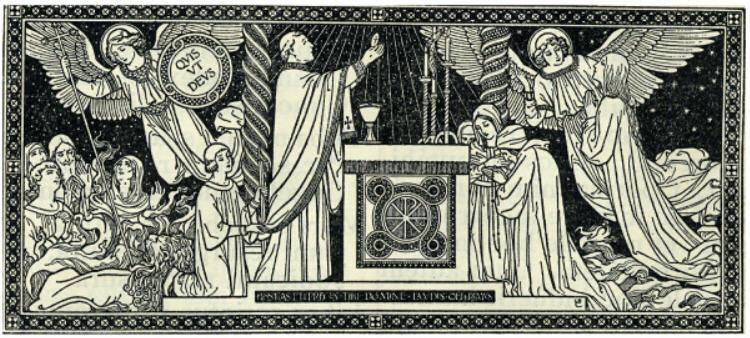
\includegraphics[width=\linewidth]{3.jpg}
\end{figure}

\section{MSZA ŚWIĘTA WIGILII PIĘCDZIESIĄTNICY}

\rubric{Odnowiwszy w sobie łaskę Chrztu, który nas wszczepił w misterium śmierci
	i Zmartwychwstania Pańskiego, składamy ofiarę Mszy świętej, W tej Ofierze w
	sakramentalny sposób stanie się obecne misterium paschalne, to jest
	tajemnicze przejście Chrystusa przez śmierć do nowego życia. Kapłan i
	usługujący ubrani w szaty mszalne koloru czerwonego udają się procesyjnie do
	ołtarza. W tym czasie chór kontynuuje Litanię, aż do końcowego Kyrie
	eleison. Teksty mszalne wysławiają działanie Ducha Świętego w duszy
	ochrzczonego i bierzmowanego. Działanie Ducha Św. Podobne jest do światła
	rozpraszającego ciemność i wody podtrzymującej życie na ziemi. Po okadzeniu
	ołtarza i odmówieniu Kyrie celebrans intonuje uroczyste Gloria, w podobny
	sposób jak w Wigilię Paschalną. Podczas hymnu dzwonią wszystkie dzwony.}

\bigskip


\oremus{Kolekta}{Præsta, quæsumus, omnípotens Deus: ut claritatis tuæ super nos
	splendor effúlgeat; et lux tuæ lucis corda eórum, qui per grátiam tuam
	renáti sunt, Sancti Spíritus illustratióne confírmet.}{Wszechmogący Boże,
	spraw, niech zabłyśnie nad nami blask Twojej chwały, a światło Twej jasności
	niechaj umocni oświeceniem Ducha Świętego tych, którzy odrodzili się przez
	łaskę.}

\proroctwoo{Epistoła (Dz 19:1--8)}
{Uczniowie Jana Chrzciciela w Efezie przyjmują chrzest}

\oremuss{In diébus illis: Factum est, cum Apóllo esset Corínthi, ut Paulus,
	peragrátis superióribus pártibus, veníret Ephesum et inveníret quosdam
	discípulos: dixítque ad eos: Si Spíritum Sanctum accepístis credéntes? At
	illi dixérunt ad eum: Sed neque, si Spíritus Sanctus est, audívimus. Ille
	vero ait: In quo ergo baptizáti estis? Qui dixérunt: In Ioannis baptísmate.
	Dixit autem Paulus: Ioánnes baptizávit baptísmo p\oe niténtiæ pópulum,
	dicens: In eum, qui ventúrus esset post ipsum, ut créderent, hoc est in
	Iesum. His audítis, baptizáti sunt in nómine Dómini Iesu. Et cum ímposuísset
	illis manus Paulus, venit Spíritus Sanctus super eos, et loquebántur
	linguis, et prophetábant. Erant autem omnes viri fere duódecim. Introgréssus
	autem synagógam, cum fidúcia loquebátur per tres menses, dísputans et
	suádens de regno Dei.}{W owym czasie, kiedy Apollos znajdował się w
	Koryncie, Paweł przeszedł okolice wyżej położone, przybył do Efezu i znalazł
	jakichś uczniów. Zapytał ich: «Czy otrzymaliście Ducha Świętego, gdy
	przyjęliście wiarę?» A oni do niego: «Nawet nie słyszeliśmy, że istnieje
	Duch Święty». «Jaki więc chrzest przyjęliście?» - zapytał. A oni
	odpowiedzieli: «Chrzest Janowy». «Jan udzielał chrztu nawrócenia,
	przemawiając do ludu, aby uwierzyli w Tego, który za nim idzie, to jest
	Jezusa» - powiedział Paweł. Gdy to usłyszeli, przyjęli chrzest w imię Pana
	Jezusa. A kiedy Paweł włożył na nich ręce, Duch Święty zstąpił na nich.
	Mówili też językami i prorokowali. Wszystkich ich było około dwunastu
	mężczyzn. Następnie wszedł do synagogi i odważnie przemawiał przez trzy
	miesiące rozprawiając i przekonując o królestwie Bożym.}

\oremus{Alleluja (Ps 106:1, 116:1--2)}{\vv Confitémini Dómino, quóniam bonus:
	quóniam in s\ae culum misericordia eius. Laudáte Dóminum, omnes gentes: et
	collaudáte eum, omnes pópuli, \\
	\vv Quóniam confirmáta est super nos misericórdia eius: et véritas Dómini
	manet in ætérnum.}{\vv Sławcie Pana, bo jest dobry, bo na wieki miłosierdzie
	Jego. Chwalcie Pana, wszystkie narody, wysławiajcie Go, wszystkie ludy.\\
	\vv Bo Jego miłosierdzie nad nami utwierdzone, a wierność Pańska trwa na wieki.}

\proroctwoo{Ewangelia (J 14:15--21)}{Duch Prawdy pozostanie z uczniami Jezusa}

\oremuss{In illo témpore: Dixit Iesus discípulis suis: Si dilígitis me, mandáta
	mea serváte. Et ego rogábo Patrem, et alium Paráclitum dabit vobis, ut
	máneat vobíscum in ætérnum, Spíritum veritátis, quem mundus non potest
	accípere, quia non videt eum nec scit eum. Vos autem cognoscétis eum: quia
	apud vos manébit et in vobis erit. Non relínquam vos órphanos: véniam ad
	vos. Adhuc módicum: et mundus me iam non videt. Vos autem vidétis me, quia
	ego vivo, et vos vivétis, In illo die vos cognoscétis, quia ego sum in Patre
	meo, et vos in me, et ego in vobis. Qui habet mandáta mea et servat ea: ille
	est, qui díligit me. Qui autem díligit me, diligétur a Patre meo: et ego
	díligam eum, et manifestábo ei meípsum.}{W owym czasie rzekł Jezus swoim
	uczniom: «Jeż eli Mnie miłujecie, będziecie zachowywać moje przykazania. Ja
	zaś będę prosił Ojca, a innego Pocieszyciela da wam, aby z wami był na
	zawsze - Ducha Prawdy, którego ś wiat przyjąć nie moż e, ponieważ Go nie
	widzi ani nie zna. Ale wy Go znacie, ponieważ u was przebywa i w was będzie.
	Nie zostawię was sierotami: Przyjdę do was. Jeszcze chwila, a ś wiat nie
	będzie już Mnie oglądał. Ale wy Mnie widzicie, ponieważ Ja żyję i wy żyć
	będziecie. W owym dniu poznacie, ż e Ja jestem w Ojcu moim, a wy we Mnie i
	Ja w was. Kto ma przykazania moje i zachowuje je, ten Mnie miłuje. Kto zaś
	Mnie miłuje, ten będzie umiłowany przez Ojca mego, a również Ja będę go
	miłował i objawię mu siebie».}

\oremus{Offertorium (Ps 103:30--31)}{Emítte Spíritum tuum, et creabúntur, et
	renovábis fáciem terræ: sit glória Dómini in s\ae cula, allelúia.}{Ześlij
	Ducha Twojego, a powstanie życie i odnowisz oblicze ziemi: niech chwała
	Pańska trwa na wieki, alleluja.}

\oremus{Pieśń}{
	1. Pamiątkę dnia świątecznego\\
	Zesłania Ducha Świętego\\
	Dziś z Kościołem obchodzimy\\
	Dawcę darów pieśnią czcimy\\
	Alleluja, alleluja.\\

	2. Co Ezechiel zwiastował,\\
	O czym Joel prorokował\\
	To na oczy wszelkie ciało\\
	W dzień świąteczny oglądało. All.\\

	3. Gdy Apostołowie mili \\
	W tym dniu rzem się modlili,\\
	Nad nimi się płomieniste\\
	Jawią języki ogniste. All.}{
	4. Boskim ogniem zapaleni,\\
	Duchem Swiętym napełnieni,\\
	Śmiało Wśród tłumu wielkiego\\
	Głoszą Ukrzyżowanego. All.\\ \\

	5. Święty Piotr jednym kazaniem,\\
	Ducha Świętego działaniem,\\
	Tak porusza słuchające,\\
	Że nawraca trzy tysiące. All.\\

	6. Dziwują się Elamici,\\
	Z ziem dalekich prozelici\\
	I Partowie i Medowie,\\
	Że ich słyszą w swojej mowie. All.}

\oremus{Sekreta}{Múnera, qu\ae sumus, Dómine, obláta sanctífica: et corda nostra
	Sancti Spíritus illustratióne emúnda.}{Prosimy Cię, Panie, uświęć złożone
	dary i oczyść nasze serca światłem Ducha Świętego.}

\oremus{Prefacja o Duchu Świętym}{Vere dignum et iustum est, æquum et salutáre,
	nos tibi semper et ubíque grátias ágere: Dómine sancte, Pater omnípotens,
	ætérne Deus: per Christum, Dóminum nostrum. Qui, hodiernia die ascéndens
	super omnes c\oe los \textbf{sedénsque ad déxteram tuam, promíssum Spíritum
		Sanctum in fílios adoptiónis effúdit}. Quaprópter profúsis gáudiis totus in
	orbe terrárum mundus exsúltat. Sed et supérnæ Virtútes atque angélicæ
	Potestátes hymnum glóriæ tuæ cóncinunt, sine fine dicéntes:}{Zaprawdę godne
	to i sprawiedliwe, słuszne i zbawienne, abyśmy zawsze i wszędzie Tobie
	składali dziękczynienie, Panie, Ojcze święty, wszechmogący, wieczny Boże:
	przez Chrystusa, Pana naszego. On to wstąpiwszy ponad wszystkie niebiosa
	\textbf{i siedząc na prawicy Twojej zesłał w dniu dzisiejszym obiecanego
		Ducha Świętego na przybrane dzieci}. Dlatego cały okrąg ziemi tonie w
	nadmiarze radości. Lecz i Moce niebieskie, i anielskie Potęgi śpiewają hymn
	ku Twojej chwale, wołając bez końca:}

\rubric{W Kanonie następujące modlitwy ulegają zmianie:}

\oremuss{Communicántes, \textbf{et diem sacratíssimum Pentecóstes celebrántes},
	quo Spíritus Sanctus Apóstolis innúmeris linguis appáruit: sed et memóriam
	venerántes...\\ \\  \\
	Hanc igitur oblationem servitutis nostræ, set et cunctæ familiæ tuæ, quam
	tibi offerimus pro his quoque, \textbf{quos regenerare dignatus es ex aqua,
		et Spiritu Sancto, tribuens eis remissionem omnium peccatorum}, quǽsumus
	Domine, ut placatus accipias: diesque nostros in tua pace disponas, atque ab
	æterna damnatione nos eripi, et in electorum tuorum iubeas grege numberari.
	Per Christum Dominum nostrum. Amen.}{Zjednoczeni w Świętych Obcowaniu,
	\textbf{obchodzimy prześwięty dzień Pięćdziesiątnicy}, w którym Duch Święty
	ukazał się Apostołom pod postacią niezliczonych języków, i ze czcią
	wspominamy...\\ \\
	Prosimy Cię przeto, Panie, abyś łaskawie przyjął tę ofiarę od nas sług
	Twoich, jak również od całego ludu Twego; składamy Ci ją za tych także,
	\textbf{których raczyłeś odrodzić z wody i Ducha Świętego, udzielając im
		odpuszczenia wszystkich grzechów}; racz dni nasze pokojem swym napełnić, od
	potępienia wiecznego nas uchronić i do grona wybranych swoich zaliczyć. Przez
	Chrystusa, Pana naszego. Amen.}

\oremus{Communio (J 7:37--39)}{Ultimo festivitátis die dicébat Iesus: Qui in me
	credit, flúmina de ventre eius fluent aquæ vivæ: hoc autem dixit de Spíritu,
	quem acceptúri erant credéntes in eum, allelúia, allelúia.}{W ostatnim dniu
	święta mówił Jezus: Kto wierzy we mnie, rzeki wody żywej popłyną z jego
	wnętrza. A to mówił o Duchu, którego otrzymać mieli wierzący weń, alleluja.}

	% \vspace*{0.5cm}

	\centerline{\pgfornament[width=3cm]{106}}

	% \vspace*{0.5cm}

\newpage

\oremus{Pieśń}{
	1. Oto są baranki młode,\\
	oto ci, co zawołali alleluja!\\
	Dopiero przyszli do zdrojów,\\
	światłością się napełnili,  \\
	Alleluja, alleluja!\\

	2. Na Baranka Pańskich godach,\\
	W szat świątecznych czystej bieli,  \\
	Po krwawego morza wodach\\
	Nieśmy Panu pieśń weseli.\\

	3. W swej miłości wiekuistej\\
	On nas swoją Krwią częstuje,\\
	Nam też Ciało swe przeczyste\\
	Chrystus kapłan ofiaruje. \\

	4. Na drzwi świętą Krwią skropione\\
	Anioł mściciel z lękiem wziera,\\
	Pędzi morze rozdzielone,\\
Wrogów w nurtach swych pożera.\\}{

	5. Już nam Paschą Tyś jest Chryste,\\
	Wielkanocną też ofiarą,\\
	Tyś Przaśniki nasze czyste \\
	Dla dusz prostych z szczerą wiarą.\\\\

	6. O Ofiaro niebios święta,\\
	Ty moc piekła pokonywasz,\\
	Zrywasz ciężkie śmierci pęta,\\
Wieniec życia nam zdobywasz.\\

	7. Chrystus piekło pogromiwszy\\
	Swój zwycięski znak roztacza,\\
	Niebo ludziom otworzywszy\\
Króla mroków w więzy wtłacza.\\

	8. Byś nam wiecznie, Jezu drogi, \\
	Wielkanocną był radością,\\
	Strzeż od grzechu śmierci srogiej \\
	Odrodzonych Twą miłością.}

\vspace*{-0.5cm}

\begin{center}
	9. Chwała Ojcu i Synowi, \\
	który z martwych żywy wstaje\\
	I Świętemu też duchowi \\
	Niech na wieki nie ustaje. \\
\end{center}

\vspace*{-0.4cm}

\oremus{Pieśń}{
	1. U drzwi Twoich stoję, Panie, \textbf{x2}\\
	czekam na Twe zmiłowanie. \textbf{x2} \\

	2. Który pod postacią chleba, \\
	prawdziwy Bóg jesteś z nieba.\\

	3. W tej Hostyi jest Bóg żywy, \\
	choć zakryty, lecz prawdziwy.\\

	4. W tym Najświętszym Sakramencie, \\
	obecny w każdym momencie.\\

	5. Jak wielki cud Bóg uczynił, \\
	gdy chleb w Ciało swe przemienił.}{
	6. A nam pożywać zostawił, \\
	ażeby nas przez to zbawił.\\

	7. Święty, Mocny, Nieśmiertelny, \\
	w Majestacie Swym niezmierny.\\

	8. Aniołowie się lękają, \\
	choć na Jego twarz patrzają.\\

	9. Wszyscy niebiescy Duchowie, \\
	lękają się i królowie.\\

	10. Niebo, ziemia ani morze, \\
	pojąć, co jest Bóg, nie może.}

\newpage

\oremus{Modlitwa po Komunii}{Sancti Spíritus, Dómine, corda nostra mundet
	infúsio: et sui roris íntima aspersióne fecúndet.}{Panie, niech tchnienie
	Ducha Świętego oczyści nasze serca i użyźni je rosą Jego łaski.}

%					\centerline{\rule{3cm}{1.2pt}}

\oremus{Regina C\ae li}{
	Regina C\ae li, l\ae tare, alleluia, \\
	Quia quem meruisti portare, alleluia, \\
	Resurrexit, sicut dixit, alleluia, \\
	Ora pro nobis Deum, alleluia.}{
	Królowo nieba, wesel się, alleluja, \\
	Bo Ten, któregoś nosiła, alleluja, \\
	Zmartwychwstał jak powiedział, alleluja, \\
	Módl się za nami do Boga, alleluja.}

\vfill

\oremus{Pieśń}{}{}

Przez Twoje święte Ducha Zesłanie, Boży Synu! odpuść nam nasze zgrzeszenie: \\
Wierzymy żeś Ducha zesłał, Żywoteś nas naprawił; \\
Śmierci wiecznej nas zbawił, Śwoję świętą moc zjawił.

% \vspace*{1cm}

% \centerline{\pgfornament[width=7cm]{82}}

\end{document}







